\chapter{Analyse}

\section{Recherche}

\subsubsection{Bezeichnung}
Der Ausdruck \gls{glos:droneLabel} kommt vom niederdeutschen Wort \textit{"`drone"'}, welches wiederrum seine Ursprung beim indogermanischen Wort \textit{"`dhren"'} hat. Die Bedeutung dieses Wortes lautet "`brummen"' oder "`dröhnen"'. \footcite{Geschichte_der_Drohne_-_Nachrichten_Print_-_DIE_WELT_-_Wissen_Print_DW_-_DIE_WELT_2015-03-21}

\begin{framed}
	\textit{Definition: }\textbf{\gls{glos:droneLabel}}\\
	Als \gls{glos:droneLabel} wird ein unbemanntes Luftfahrzeug bezeichnet. Die Steuerung kann entweder manuell oder autonom erfolgen.\\
	Quelle: 
	\cite{Drone_Define_Drone_at_Dictionary.com_2015-03-21}
\end{framed}

\subsection{Geschichte der Drohne}
% http://www.informatik.uni-oldenburg.de/~iug08/snd/geschichte1.html
% http://diepresse.com/home/politik/innenpolitik/1385181/Die-Geschichte-der-Drohnen
% http://www.welt.de/print/welt_kompakt/print_lifestyle/article135929763/Kleine-Geschichte-der-Drohnen.html
% http://www.welt.de/print/die_welt/wissen/article127106535/Geschichte-der-Drohne.html
% http://de.wikipedia.org/wiki/Unbemanntes_Luftfahrzeug
% http://de.wikipedia.org/w/index.php?title=Autonomes_Luftfahrzeug&action=edit&redlink=1
% http://en.wikipedia.org/wiki/History_of_unmanned_aerial_vehicles

\subsection{Frühe Entwicklung}
Eine der allerersten bekannten \gls{glos:droneLabel} war wohl, 1783 von den Brüder Mongolfier aus Frankreich, ein unbemannter Heissluftballon. \footcite{Kleine_Geschichte_der_Drohnen_-_Nachrichten_Print_-_WELT_KOMPAKT_-_Lifestyle_-_DIE_WELT_2015-03-21}
\footcite{Unbemannte_Luftfahrt__Wikipedia_2015-03-22}

\subsection{Waffenträger}
Anschliessend wurde das Potenzial von \glspl{glos:droneLabel} besonders für kriegerische Zwecke erforscht und entwickelt.

\begin{wrapfigure}{r}{0.4\textwidth}
	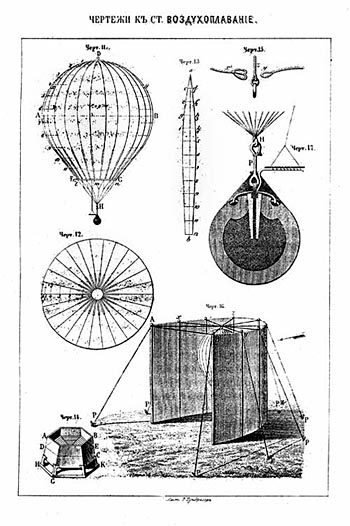
\includegraphics[width=1.0\linewidth]{images/analysis/balloonbombs1849.jpg}
 	\caption[Bombing by Balloon, 1848]{Bombing by Balloon, 1848 \protect\footcite{Remote_Piloted_Aerial_Vehicles_2015-03-21}}
\end{wrapfigure}

So wurden bereits 1849, vom österreichischen Königsreich, unbemannte Heissluftballons mit Bomben im Krieg gegen Venedig losgeschickt.
Weder die "`\gls{glos:droneLabel}"' selbst, noch das Abwerfen der Bombe konnten aktiv gesteuert werden.
Die Heissluftballons flogen mit dem Wind und die Bomben wurde per Zeitzünder gezündet. Tatsächlich erreichten einzelne Ballons ihr Ziel und konnten Schaden anrichten, andere jedoch wurden vom Wind zurück geweht und zerstörten das eigene Territorium Österreichs. \footcite{Remote_Piloted_Aerial_Vehicles_2015-03-21}

Während des Ersten Weltkrieges wurden die ersten unbemannten Flugzeuge in Amerika entwickelt.
Mit diesen wurden vordefinierte Routen abgeflogen und es konnten \textit{Flugtorpedos} abgeworfen werden, welche wie die Flugzeuge selbst, mit Hilfe von gyroskopischen Stabilisierer und Aneroidbarometer zwar Richtung und Höhe halten konnten, jedoch nicht per Funk steuerbar waren.

Die ersten funkgesteuerten \glspl{glos:droneLabel} wurde erst nach dem Krieg 1918 fertig. Nebst den Amerikanern, hatten auch die Briten 1925 ihren ersten Drohnenflug verbucht. Diese konnte ca. 300\,Meilen (ca. 483\,km) mit einer Geschwindigkeit von 190\,mph (ca. 306\,km/h) zurücklegen.\footcite{Informatik_und_Gesellschaft_2015-03-21}

Da der Krieg vorbei war, wurden die \glspl{glos:droneLabel} für Jagd-Trainings der Armee genutzt.

Mit den Jahren wurde die \gls{glos:droneLabel} immer weiter verbessert und werden heute aktiv gegen terroristische Aktivitäten verwendet.

\subsection{Weitere Zwecke}
% http://diepresse.com/home/politik/innenpolitik/1385181/Die-Geschichte-der-Drohnen
Nebst den erwähnten Waffenträger gibt es auch diverse weitere Aufgaben für \glspl{glos:droneLabel}.
Besonders für Beobachtungen werden sie sehr häufig gebraucht (z.B. Aufklärung, Luftaufnahmen, Wetterbeobachtung, Transporte, Filmproduktionen), aber auch für Messungen an Orten die für Menschen ungeeignet oder schädlich sind.

Obschon jene Aufgabenbereiche gewaltfrei sind, dienen \glspl{glos:droneLabel} trotzdem mehrheitlich polizeilichen und militärischen Organisationen.\footcite{Die_Geschichte_der_Drohnen_DiePresse.com_2015-03-21}

\subsection{Heutige Einsätze von Drohnen}
Seit 2013 werden, in Grand Forks County im US-Bundesstaat North Dakota, \glspl{glos:droneLabel} zur Verbrecherjagd eingesetzt, resp. zur Suche der Personen.

Auch Amazon verkündet ihren \textit{Prime Air}-Service, der Pakete direkt vor die Haustüre liefert.

Im Jahr 2014 wurde der Einsatz für landwirtschaftliche Zwecke erprobt und auch die \gls{glos:dhlLabel} führt Testlieferungen mit \glspl{glos:droneLabel} aus.\footcite{Kleine_Geschichte_der_Drohnen_-_Nachrichten_Print_-_WELT_KOMPAKT_-_Lifestyle_-_DIE_WELT_2015-03-21}


\subsection{Flugeigenschaften von Drohnen}



\subsection{Bereits bestehende Arbeiten}

\subsubsection{Steuermöglichkeiten}

\subsubsection{Sensoren Integration auf bestehende Steuerungen}

%%% 

\section{Ist-Analyse}
\subsection{Gestensensor}

\subsubsection{Einsatz}

\subsubsection{Technische Details}

\subsubsection{API}


\subsection{Drohne}

\subsubsection{API}
% \subsubsection{Sensoren charakterisieren}

%%% 

\section{Soll-Analyse}
\subsection{Gesten-Steuerbeschrieb}


%%% 
